\section{Auswertung}

Die notierten Gerätedaten lauten:

\begin{itemize}
  \item L = \SI{3.53(3)}{\milli\H}
  \item C = \SI{5.015(15)}{\nano\F}
  \item $R_1$ = \SI{30.3(1)}{\ohm}
  \item $R_2$ = \SI{271.6(3)}{\ohm}
\end{itemize}

Zunächst wird eine gedämpfte Schwingung mithilfe eines RCL-Kreises untersucht.
Die Messwerte der Minima und Maxima sind in Tabelle (\ref{tab:1}) dargestellt und in
Abbildung (\ref{fig:6}) wird der Thermodruck des Oszilloskopes gezeigt. $U_0$ ist die Spannung
des Generators und in diesem Fall beträgt sie $1,18\si{\V}$.

\begin{table}[H]
  \centering
  \caption{Messwerte einer gedämpften Schwingung.}
  \label{tab:1}
  \begin{tabular}{c c c c c c}
    \toprule
    \multicolumn{3}{c}{Maxima} & \multicolumn{3}{c}{Minima} \\
    \cmidrule(lr){1-3}\cmidrule(lr){4-6}
    $U / \si{\V}$ & $\frac{U}{U_0}$ & $t / \si{\second}$ & $U / \si{\V}$ & $\frac{U}{U_0}$ & $t / \si{\second}$ \\
    \midrule
    3,2     & 2,02  &    4 & -0,52 &  -1,7   &  18 \\
    2,64    & 1,46  &   32 & -0,08 &  -1,26  &  44 \\
    2,26    & 1,08  &   58 & 0,28 &  -0,9   &  72 \\
    1,96    & 0,78  &   86 & 0,52 &  -0,66  &  98 \\
    1,76    & 0,58  &  112 & 0,7 &  -0,48  & 126 \\
    1,6     & 0,42  &  140 & 0,86 &  -0,32  & 152 \\
    1,5     & 0,32  &  166 & 0,94 &  -0,24  & 180 \\
    1,44    & 0,26  &  194 & 1 &  -0,18  & 208 \\
    1,36    & 0,18  &  220 & 1,08 &  -0,10  & 234 \\
    1,3     & 0,12  &  248 & 1,1 &  -0,08  & 260 \\
    1,26    & 0,08  &  274 & 1,14 &  -0,04  & 288 \\
    1,24    & 0,06  &  302 & 1,16 &  -0,02  & 316 \\
    \bottomrule
  \end{tabular}
\end{table}

\begin{figure}[H]
  \centering
  \caption{Thermodruck einer gedämpften Schwingung.}
  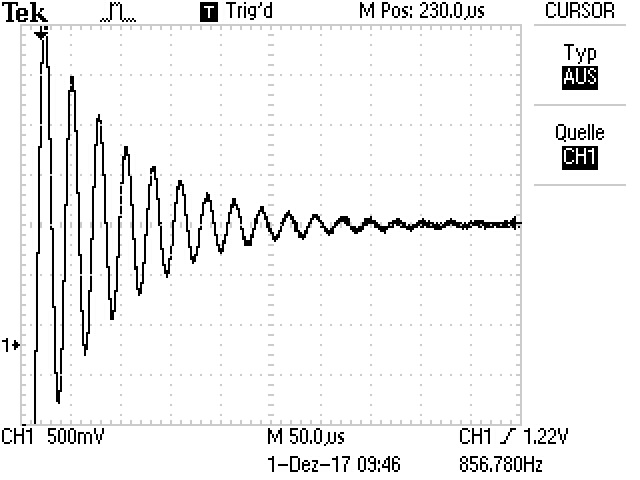
\includegraphics[width=\textwidth]{Kurve.jpg}
  \label{fig:6}
\end{figure}

Zu diesen Messwerten lassen sich nun zwei nicht lineare Ausgleichsrechnungen durchführen,
für die Minima und die Maxima. Für die Ausgleichsrechnungen werden folgende Gleichungen
verwendet:

\begin{gather*}
  y = a \cdot \exp(-bx) \\
  y = c \cdot \exp(-dx)
\end{gather*}

Die Ausgleichsrechnung wird mit Python 3.6 durchgeführt. In Abbildung (\ref{fig:7})
ist die Ausgleichsrechnung graphisch dargestellt.

\begin{itemize}
  \item a = \SI{2.109(11)}{\V}
  \item b = \SI{11450.50(9646)}{\per\second}
  \item c = \SI{-1.809(20)}{\V}
  \item d = \SI{12049.80(21247)}{\per\second}
\end{itemize}

\begin{figure}[H]
  \centering
  \caption{Darstellung der Messwerte und der Ausgleichsrechnung für die gedämpfte Schwingung.}
  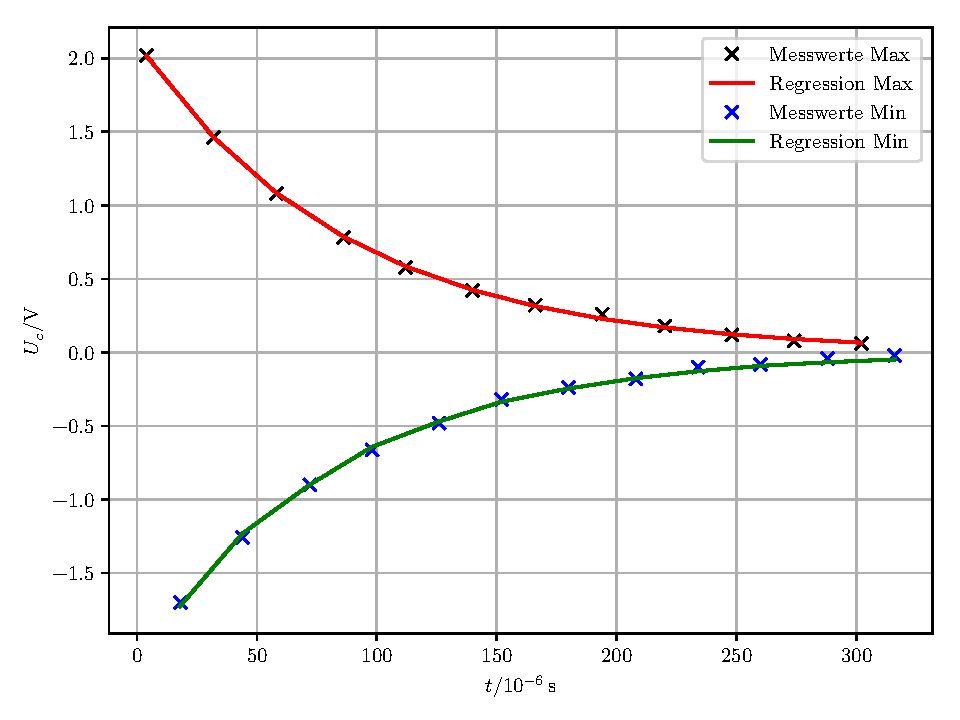
\includegraphics[width=\textwidth]{plot1.pdf}
  \label{fig:7}
\end{figure}

Durch Vergleichen der Gleichungen für die Ausgleichsrechnung und der Gleichung ()
folgt für den effektiven Dämpfungswiederstand:

\begin{equation*}
  b = \frac{R_{eff}}{2L} \iff R_{eff} = 2bL
\end{equation*}

Die Fehler werden mit der Gauß´schen Fehlerfortpflanzung bestimmt:\\\\

$\Delta R_{eff} = \sqrt{(2L \cdot \Delta b)^2 + (2b \cdot \Delta L)^2}$.\\\\

Damit ergibt sich für die Maxima:

\begin{equation*}
  R_{eff} = \SI{80.8(10)}{\ohm}.
\end{equation*}

Der eingebaute Widerstand hat $R = \SI{30.3(1)}{\ohm}$, damit ergibt sich eine Abweichung
von $\SI{50.5}{\ohm}$.

Die Rechnung für die Minima ist die selbe.

\begin{equation*}
  R_{eff} = \SI{85.1(17)}{\ohm}
\end{equation*}

Bei dieser Rechnung ergibt sich eine Abweichung von $\SI{54.8}{\ohm}$.


Mithilfe der Gleichung () lässt sich nun auch die Abklingdauer bestimmen.

\begin{equation*}
  T_{ex} = \frac{1}{2\pi\mu} = \frac{1}{b}
\end{equation*}

Für die Maxima ergibt sich somit:

\begin{equation*}
  T_{ex} = \SI{8.73(7)e-5}{\second}.
\end{equation*}

Analog für die Minima:

\begin{equation*}
  T_{ex} = \SI{8.30(15)e-5}{\second}.
\end{equation*}


Bei der Bestimmung des Widerstandes für den aperiodischen Grenzfall, wurde folgender
Widerstand durch Messungen ermittelt:

\begin{equation*}
  R_{ap} = 2810 \si{\ohm}
\end{equation*}

Durch Umformung der Gleichung () lässt sich dieser Widerstand auch theoretisch bestimmen.

\begin{equation*}
  \iff R_{ap} = \sqrt{\frac{4L}{C}}
\end{equation*}

Der Fehler wird wieder mit der Gauß´schen Fehlerfortpflanzung bestimmt:

\begin{equation*}
  \Delta R_{ap} = \sqrt{\left( \frac{2}{\sqrt{4LC}}\cdot \Delta L\right)^2 +
  \left( \frac{-\sqrt{4L}}{2C^{\frac{3}{2}}}\cdot \Delta C \right)^2}
\end{equation*}

Nun folgt für den theoretisch bestimmten Widerstand $R_{ap} = \SI{1678(8)}{\ohm}$,
es gibt also eine Abweichung von $67,64 \% $.


Daraufhin wird die Kondensatorspannung in Abhängigkeit von der angelegten Spannungsfrequenz
untersucht. In der Abbildung (\ref{fig:8}) ist die relative Kondensatorspannung und die
Frequenz halblogarithmisch aufgetragen. Die Generatorspannung ist dabei konstant
$ U_0 = \SI{1.3}{\V}$.

\begin{figure}[H]
  \centering
  \caption{Messwerte der relativen Kondensatorspannung bei einer angelegten Sinusspannung.}
  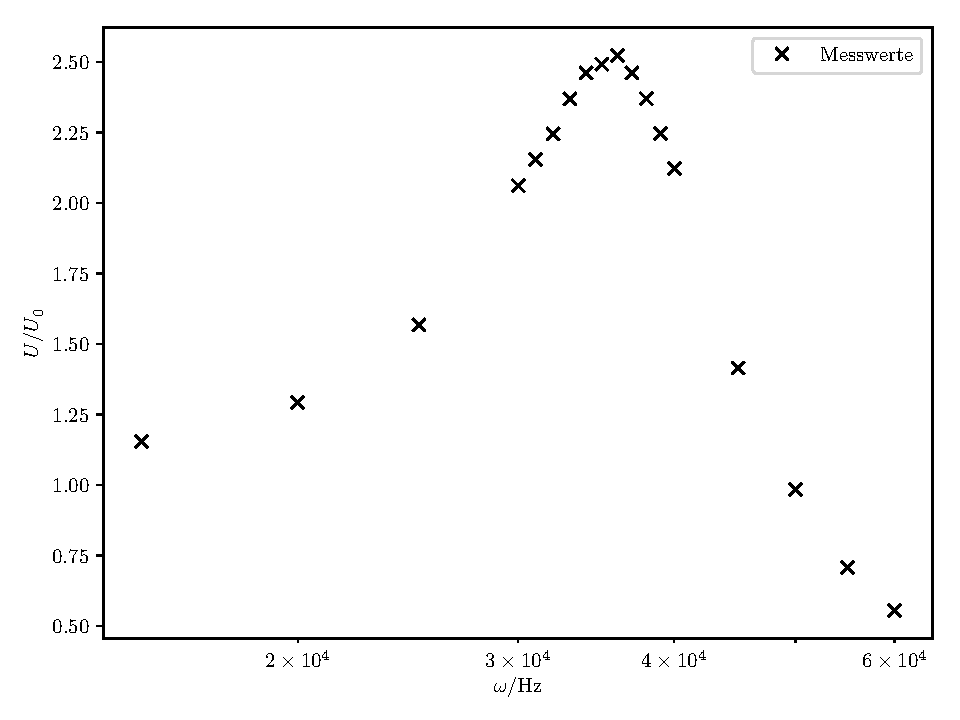
\includegraphics[width=\textwidth]{plot2.pdf}
  \label{fig:8}
\end{figure}

\begin{table}[H]
  \centering
  \caption{Tabelle mit den Messdaten zur bestimmung der Resonanzüberhöhung.}
  \label{tab:2}
  \begin{tabular}{c c c}
    \toprule
    $U/\si{\V}$ & $\frac{U}{U_0}$ & $ \omega / \si{\Hz}$ \\
    \midrule
    1,5  & 1,154 &  15000 \\
    1,68 & 1,292 &  20000 \\
    2,04 & 1,569 &  25000 \\
    2,68 & 2,062 &  30000 \\
    2,8  & 2,154 &  31000 \\
    2,92 & 2,246 &  32000 \\
    3,08 & 2,369 &  33000 \\
    3,2  & 2,462 &  34000 \\
    3,24 & 2,492 &  35000 \\
    3,28 & 2,523 &  36000 \\
    3,2  & 2,462 &  37000 \\
    3,08 & 2,369 &  38000 \\
    2,92 & 2,246 &  39000 \\
    2,76 & 2,123 &  40000 \\
    1,84 & 1,415 &  45000 \\
    1,28 & 0,985 &  50000 \\
    0,92 & 0,708 &  55000 \\
    0,72 & 0,554 &  60000 \\
    \bottomrule
  \end{tabular}
\end{table}

Aus der Abbildung (\ref{fig:8}) lässt sich entnehmen und mithilfe der Gleichung (),
dass die Resonanzüberhöhung

\begin{equation*}
  q = \frac{U_{c,max}}{U_0} = 2,523
\end{equation*}

ist. Der theoretische Wert lässt sich mit der Gleichung () und mit dem Zusammenhang
$\omega_0 = \frac{1}{\sqrt{LC}}$ bestimmen. Damit ergibt sich dann:

\begin{equation*}
  q_{theo} = \frac{1}{R} \sqrt{\frac{L}{C}}
\end{equation*}

Die Formel für den Fehler ergibt sich mit der Gauß´schen Fehlerfortpflanzung:

\begin{equation*}
  \Delta q = \sqrt{\left( \frac{-\sqrt{L}}{R^2\sqrt{C}} \cdot \Delta R \right)^2 +
  \left( \frac{1}{2R\sqrt{LC}} \cdot \Delta L \right)^2 +
  \left( \frac{-\sqrt{L}}{2RC^{\frac{3}{2}}} \cdot \Delta C \right)^2}
\end{equation*}

Bei dieser Messung wurde der Widerstand $R_2$ benutzt. Somit ergibt sich für den theoretischen
Wert:

\begin{equation*}
  q_{theo} = \num{3.089(14)}
\end{equation*}

Die Abweichung ist damit $18,32\% $.
